\chapter{Association Analysis: Basic Concepts and Algorithms}

	This chapter presents a methodology known as {\bf association analysis},
	which is useful for discovering interesting relationships hidden in large
	data sets, such as shopping basket transactions. 
	The uncovered relationships can be represented in the form of 
	{\bf association rules} or sets of {\bf frequent items}. 

	\clearpage
	\section{Problem Definition}

	This section reviews the basic termonology used in association analysis.

		\subsection*{Binary representation} 
		market basket data can be represented in a binary
		format as shown below. Each row correspond to a transaction (TID = transactio ID)
		and each column correspond to an item. A item in a transaction have the value
		"1" if the item is present in the transaction, otherwise it is "O".
		Because the presence of an item in a transaction is often considered more
		important than its absence, an item is an {\bf asymmetric binary value}.

		\begin{figure}[H]
		\centering
			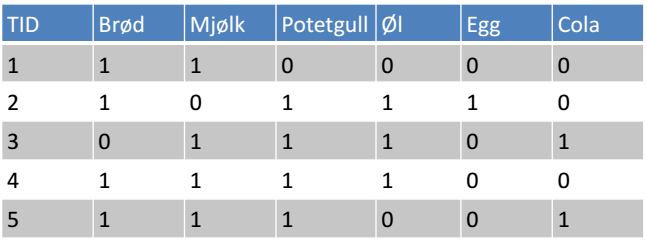
\includegraphics[scale = 0.4]{pics/binary.png}
			\caption{Binary representation of transaktions from market basket data}
		\end{figure}

		\subsection*{Itemset and support count} 
		Let $ I = \{i_{1}, i_{2}, ...., i_{d}\}$ be the
		set of all items in a market basket data and $ T = \{t_{1}, t_{2},....,t_{N}\}$
		be the set of all transactions. Each transaction $t_{i}$ contains a subset of items
		chosen from I. In assiciation analysis, a collection of zero or more items
		is termed an {\bf itemset}. If an itemset contains k items, it is called a {\bf k-itemset}.
		The {\bf transaction width} is defined as the number of items present in a transaction.
		An important property of an itemset is its {\bf support count}, which refers to the 
		number of transactions that contain a particular itemset. 

		\subsection*{Association rule and confidence} 
		An association rule is an implication expression of
		the form $X \rightarrow Y$, where X and Y are disjoint itemsets, i.e., $X \cap Y = \emptyset$.
		The strength of an association rule can be measured in terms of {\bf support} and 
		{\bf confidence}. Support determines how often a rule is applicable to a given data
		set, while confidence determines how frequently items in Y appear in transactions that
		contains X. 

		\begin{equation}
			Support, s(X \rightarrow Y) = \frac{\sigma (X \cup Y)}{N}
		\end{equation}

		\begin{equation}
			Confidence, c(X \rightarrow Y) = \frac{\sigma(X \cup Y)}{\sigma(X)}
		\end{equation}

		\clearpage

		\subsection*{Why use support and confidence?}

		Support is an iportant measure because a rule that has very low support may occur simply
		by chance, or is likely to be uninteresting from a business perspective. 
		Confidence, on the other hand, measures the realiability of the inference made by a rule.
		For a given rule {\bf X $\Rightarrow$ Y}, the higher the confidence, the more likely it 
		is for Y to be present in transactions that contain X. 

		\subsection*{Example support and confidence}
		The number is from figure 6.1. We will calculate the support and confidence for the 
		association rule {\bf \{Mjølk, Potetgull\} $\Rightarrow$ \{Øl\}}. \\
		\{Mjølk, Potetgull, Øl\} appear in 2 of the transactions and \{Mjølk, Potetgull\} is 
		appear in 3 of the transactions. The total number of transactions is 5.   
		
		\begin{equation}
			s = \frac{\sigma(Mjølk,Potetgull, Øl)}{Number of transactions} = \frac{2}{5} = 0.4
		\end{equation}
		\begin{equation}
			c = \frac{\sigma(Mjølk, Potetgull, Øl)}{\sigma(Mjølk, Potetgull)} =  \frac{2}{3} = 0.67
		\end{equation}

		\subsection*{Minsup and minconf threshold}
		Given a set of transactions T, find all the rules having support $\geq$ minsup and \\
		confidence $\geq$ minconf, where minsup and minconf are the corresponding support
		and confidence thresholds. 

		A brute-force apporach for mining association rules is to compute the support and
		confidence for every possible rule. This approach is prohibittively expensive!
		Therefore, a common strategy is to decompose the problem into two major subtasks:

		\begin{enumerate}
			\item {\bf Frequent Itemset Generation,} whose objective is to find all the 
			itemsets that satisfy the minsup threshold. These itemsets are called 
			frequent itemsets. 
			\item {\bf Rule generation,} whose objective is to extract all the high-confidence
			rules from the frequent itemsets found in the previous step. These rules
			are called {\bf strong rules}.
		\end{enumerate}

	\clearpage 
	\section{Frequent Itemset Generation}

		A lattice structure can be used to enumerate the list of all possible itemsets.
		Figure 6.2 shows an itemset lattice for I = \{a,b,c,d,e\}. The lattice shows
		all possible itemsets, also called {\bf candidate itemsets}. To calculate
		the support count for every candidate itemsets, we need to compare each candidate
		against every transaction.

		\begin{figure}[H]
			\centering
			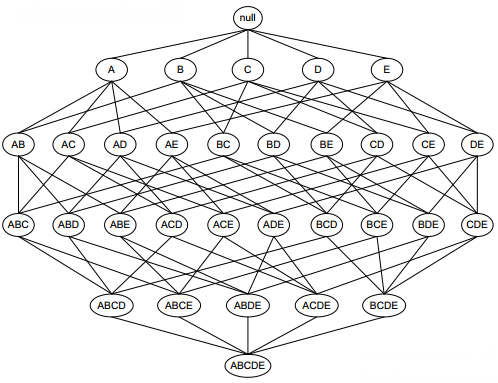
\includegraphics[scale=0.5]{pics/lattice.png}
			\caption{An itemset lattice}
		\end{figure}

		This method have a hight computational compleexity. There are several ways to reduce 
		the computitional complexity for frequent itemset generation. 

		\begin{enumerate}
			\item {\bf Reduce the number of candidate itemsets (M):} the {\it Apriori}
			princible in the next section is an very effective way to eliminate
			some of the candidate itemsets without counting their support values. 
			\item{\bf Reduce the number of comparisons:} Instead of matching each candidate
			itemset against every transaction, we can reduce the number of 
			comparisons by using more advanced data structures, either to store the
			candidate itemsets or to compress the data set. 
		\end{enumerate}

	\clearpage
	\section{The Apriori Principle}

		{\bf Apriori principle:} {\it If an itemset is frequent, then all of its subsets must also be frequent}.

		\begin{figure}[H]
			\centering
			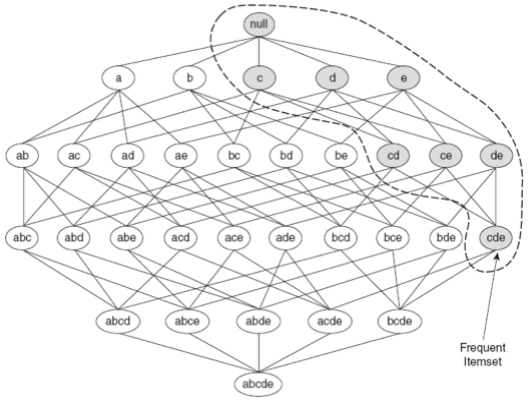
\includegraphics[scale=0.5]{pics/lattice3.png}
			\caption{Apriori principle: the itemset cde + all of its subsets is a frequent itemset}
		\end{figure}

		\begin{figure}[H]
			\centering
			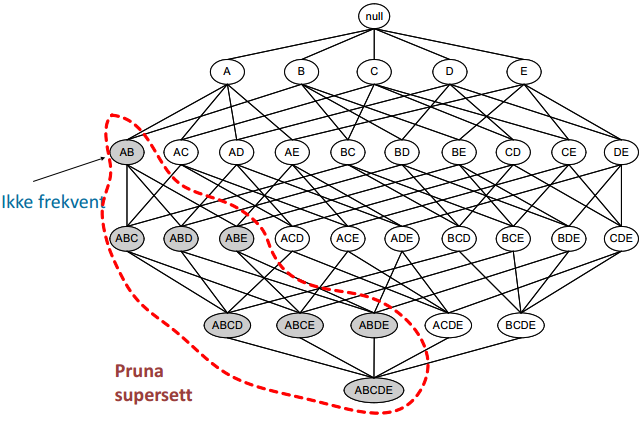
\includegraphics[scale=0.5]{pics/lattice4.png}
			\caption{Apriori principle: the itemset AB is infrequent, then all of its supersets must be infrequent}
		\end{figure}

	\clearpage

	\section{Apriori Algorithm}

		Let $C_{k}$ denote the set of candidate k-itemsets and $F_{k}$ denote the set of frequent 
		k-itemsets:

		\subsection*{The frequent itemset generation part of the Apriori algorithm}
		\begin{itemize}
			\item The algorithm initially makes a single pass over the data set to determine
			the support of each item. Upon completion of this step, the set of all frequent
			1-itemsets, $F_{1}$, will be known.
			\item Next, the algorithm will iteratively generate new candidate k-itemsets
			using the frequent (k-1)-itemsets found in the previous iteration. Candidate
			generation is implemented using a function called apriorigen.
			\item To count the support of the candidates, the algorithm needs to make 
			an additional pass over the data set. The subset function is used to determine
			all the candidate itemsets in $C_{k}$ that are contained in each transaction t.
			\item After counting their supports, the algorithm eliminates all candidate
			itemsets whose support counts are less than minsup.
			\item The algorithm terminates when there are no new frequent itemsets generated,
			i.e., ($F_{k} = \emptyset$).
		\end{itemize}

		\subsection*{Apriori-gen function}
		\begin{itemize}
			\item {\bf Candidate Generation:} this operation generates new candidate
			k-itemsets based on the frequent (k-1)-itemsets found in previous iteration.
			\item {\bf Candidate Pruning:} this operation eliminates some of the candidate
			k-itemsets using the support-based pruning strategy
		\end{itemize}

		\begin{figure}[H]
			\centering
			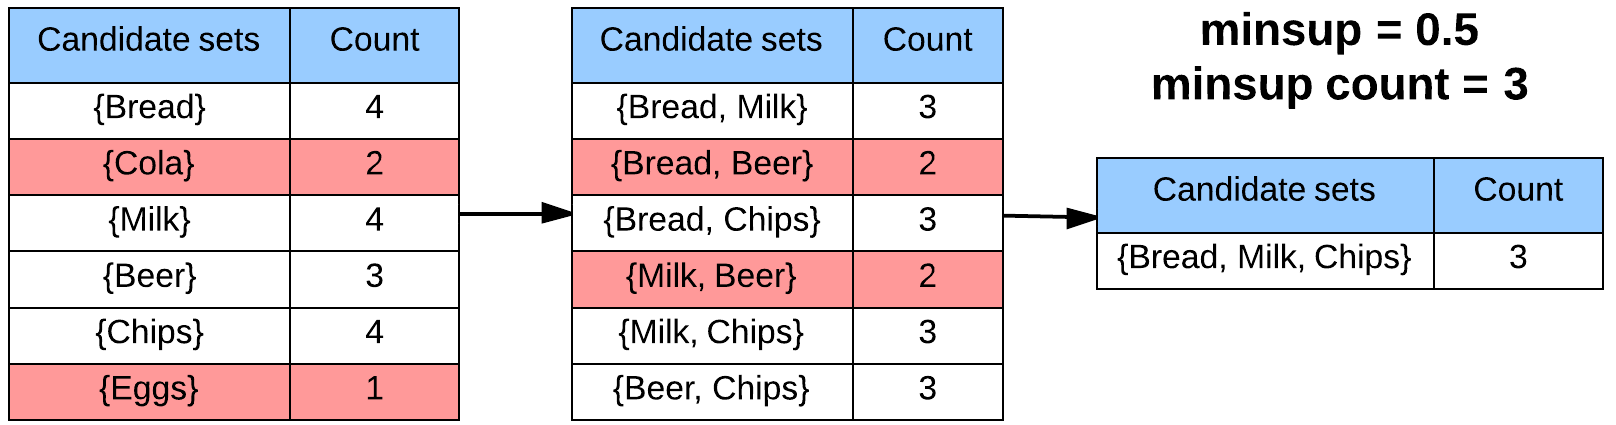
\includegraphics[width=\textwidth]{pics/apriori.png}
			\caption{Itemset generation with pruned itemsets in red}
		\end{figure}

		\subsection*{Requirements for an effective candidate generation procedure}

		\begin{enumerate}
			\item It should avoid generating too many unnecessary candidates.
			\item It must ensure that the candidate set is complete, i.e., no frequent
			itemsets are left out by the candidate generation procedure. 
			\item It should not generate the same candidate itemset more than once.
		\end{enumerate}

		\clearpage
		\section{Apriori Candidate generation procedures}

			\subsection{Brute-Force Method}
				The brute-force method considers every k-itemsets as a potential candidate and then 
				applies the candidate pruning step to remove any unnecessary candidates. 

			\subsection{$F_{k-1} \times F{1}$ Method}
				An alternative method for generation is to extend each frequent (k-1)-itemset with 
				other frequent items. This method can generate duplicate candidates. One way of
				avoid generating duplicate candidates is by ensuring that the items in each frequent 
				itemset are are kept strted in their lexicographically larger than the items in X. 
				For examplel, the itemset \{Bread, Diapers\} can be argumented with \{Milk\}
				since Milk is lexiicographically larger than Bread and Diapers. However, we
				should not augment \{Bread, Diapers\} with \{Bread\} nor \{Bread, Milk\} with 
				\{Diapers\} because they violate the lexocographic ordering condition. 
 
			\subsection{$F_{k-1} \times F_{k-1}$ Method}
				The candidate generation procedure in the apriori-gen function merges a pair of 
				frequent (k-1)-itemsets only if their first k-2 items are identical. 
				Let A = \{$a_{1}, a_{2},...,a_{k-1}$\} and B = \{$b_{1}, b_{2},...,b_{k-1}$\}
				be a pair of frequent (k-1)-itemsets. A and B are merged if they satisfy the following
				conditions:

				$a_{i} = b_{i} (for i =1, 2,..., k-2)$ and $a_{k-1} \neq b_{k-1}$

				The frequent itemsets \{Bread, Diapers\} and \{Bread, Milk\} are merged to form a 
				candidate 3-itemset \{Bread, Diapers, Milk\}. The algorithm does not have to merge
				\{Beer, Diapers\} with \{Diapers, Milk\} because the first item in both itemsets is
				different. Indeed, if \{Beer, Diapers, Milk\} is a viable candidate, it would have been
				obtained by merging \{Beer, Diapers\} with \{Beer, Milk\}.
				
				\begin{figure}[H]
					\centering
					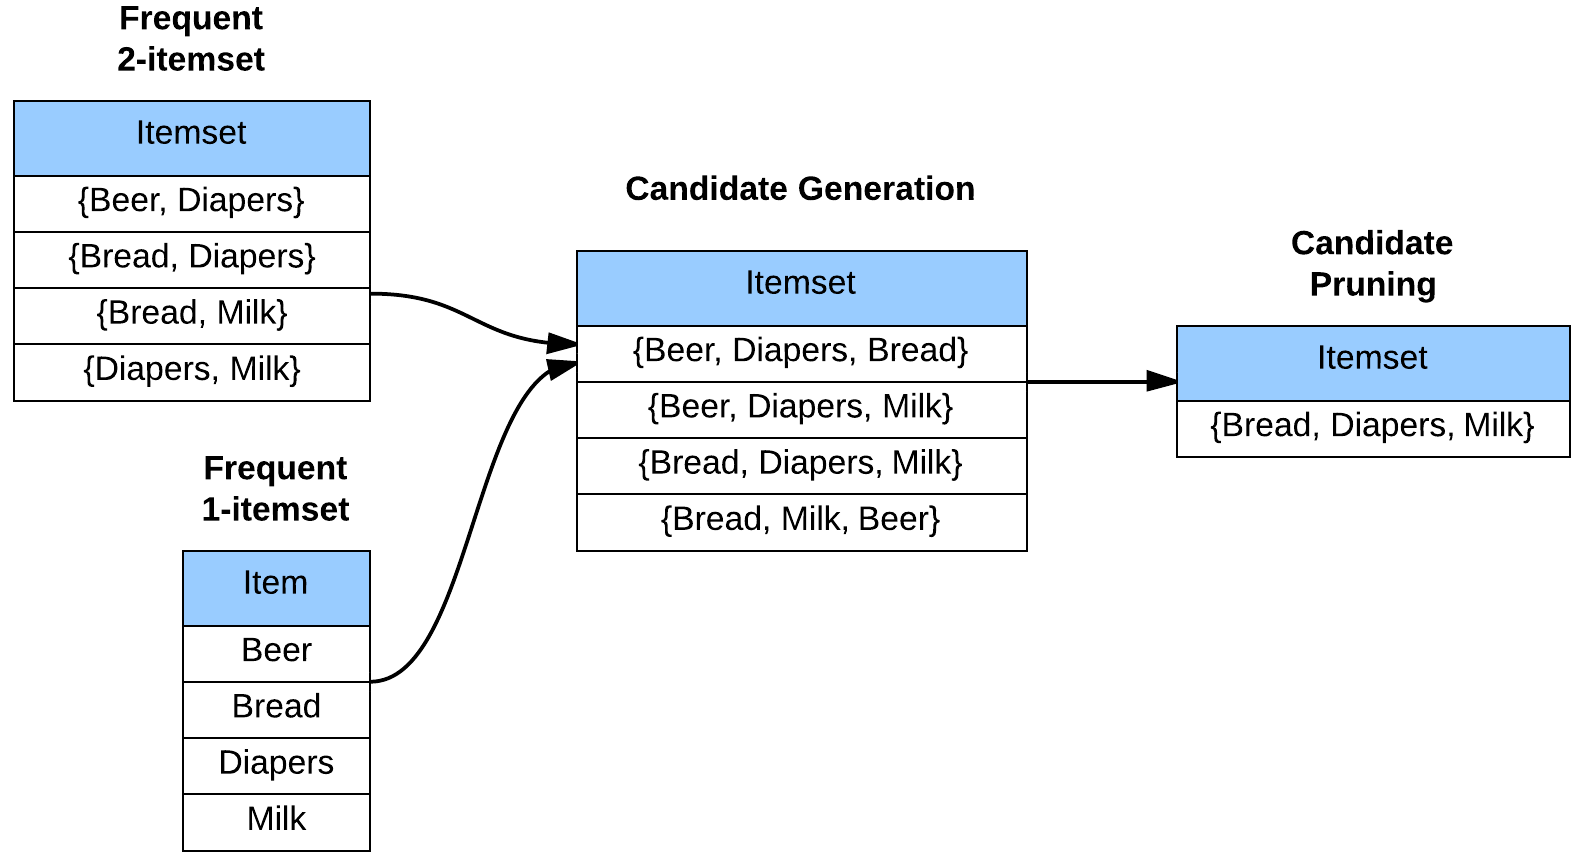
\includegraphics[width=\textwidth]{pics/apriori2.png}
					\caption{$F_{k-1} \times F{1}$ illustration}
				\end{figure}

				\begin{figure}[H]
					\centering
					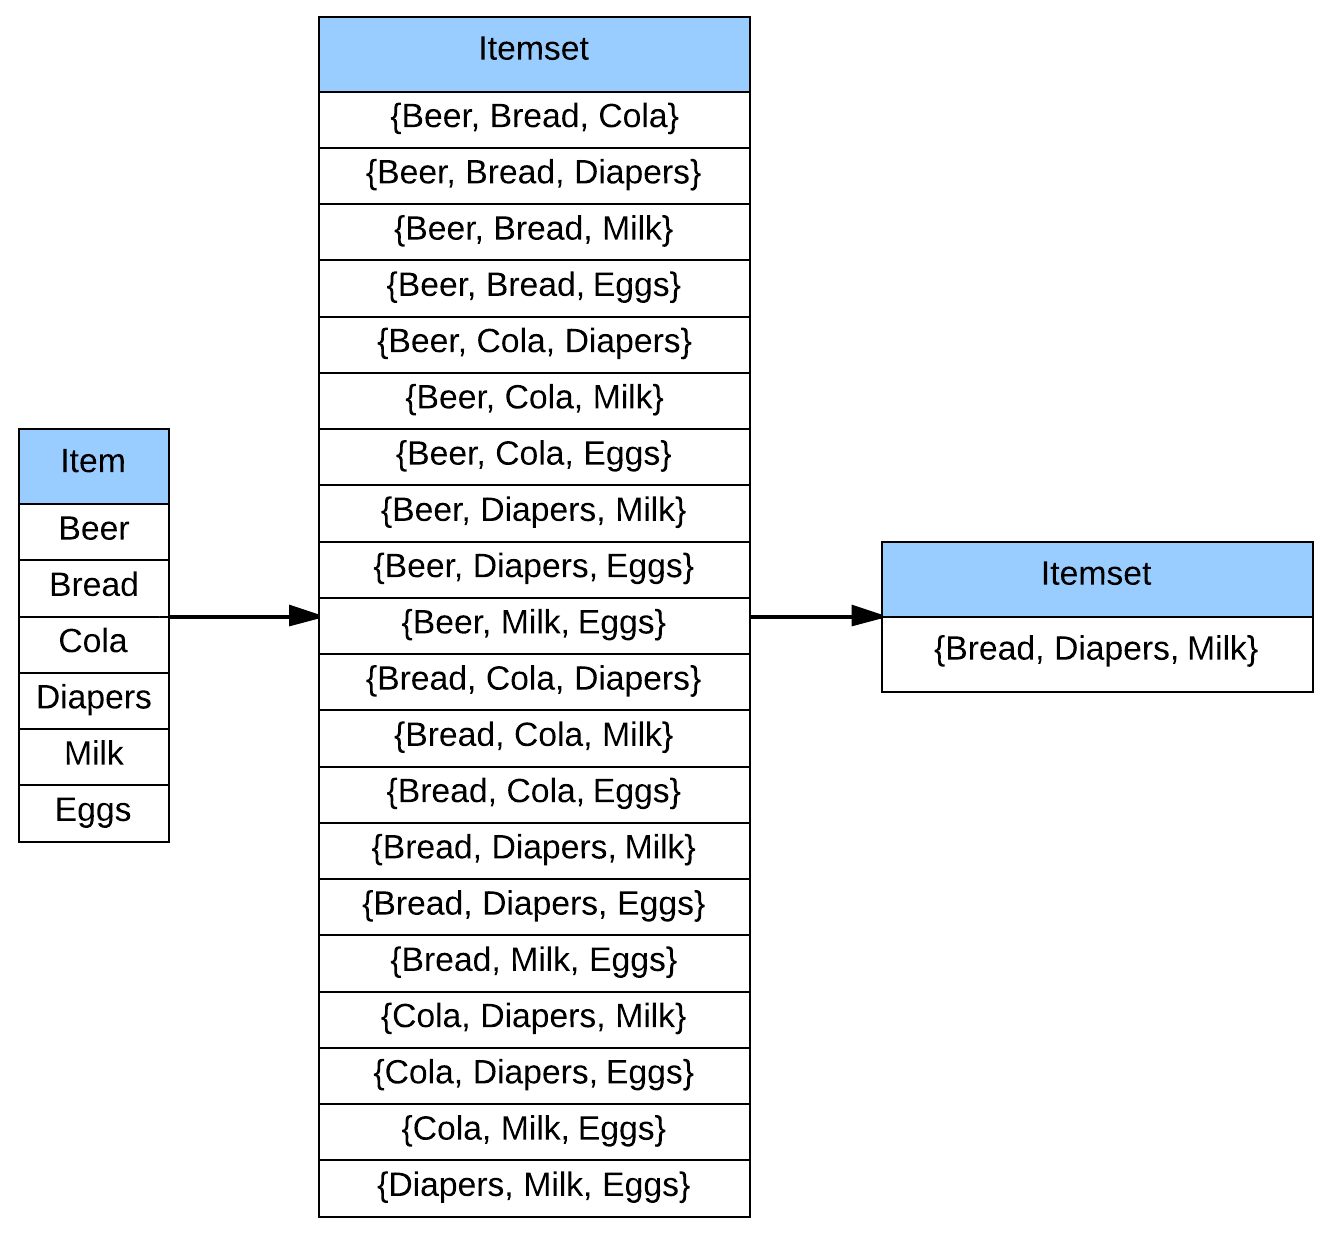
\includegraphics[scale=0.2]{pics/apriori1.png}
					\caption{Brute-Force illustration}
				\end{figure}

				\begin{figure}[H]
					\centering
					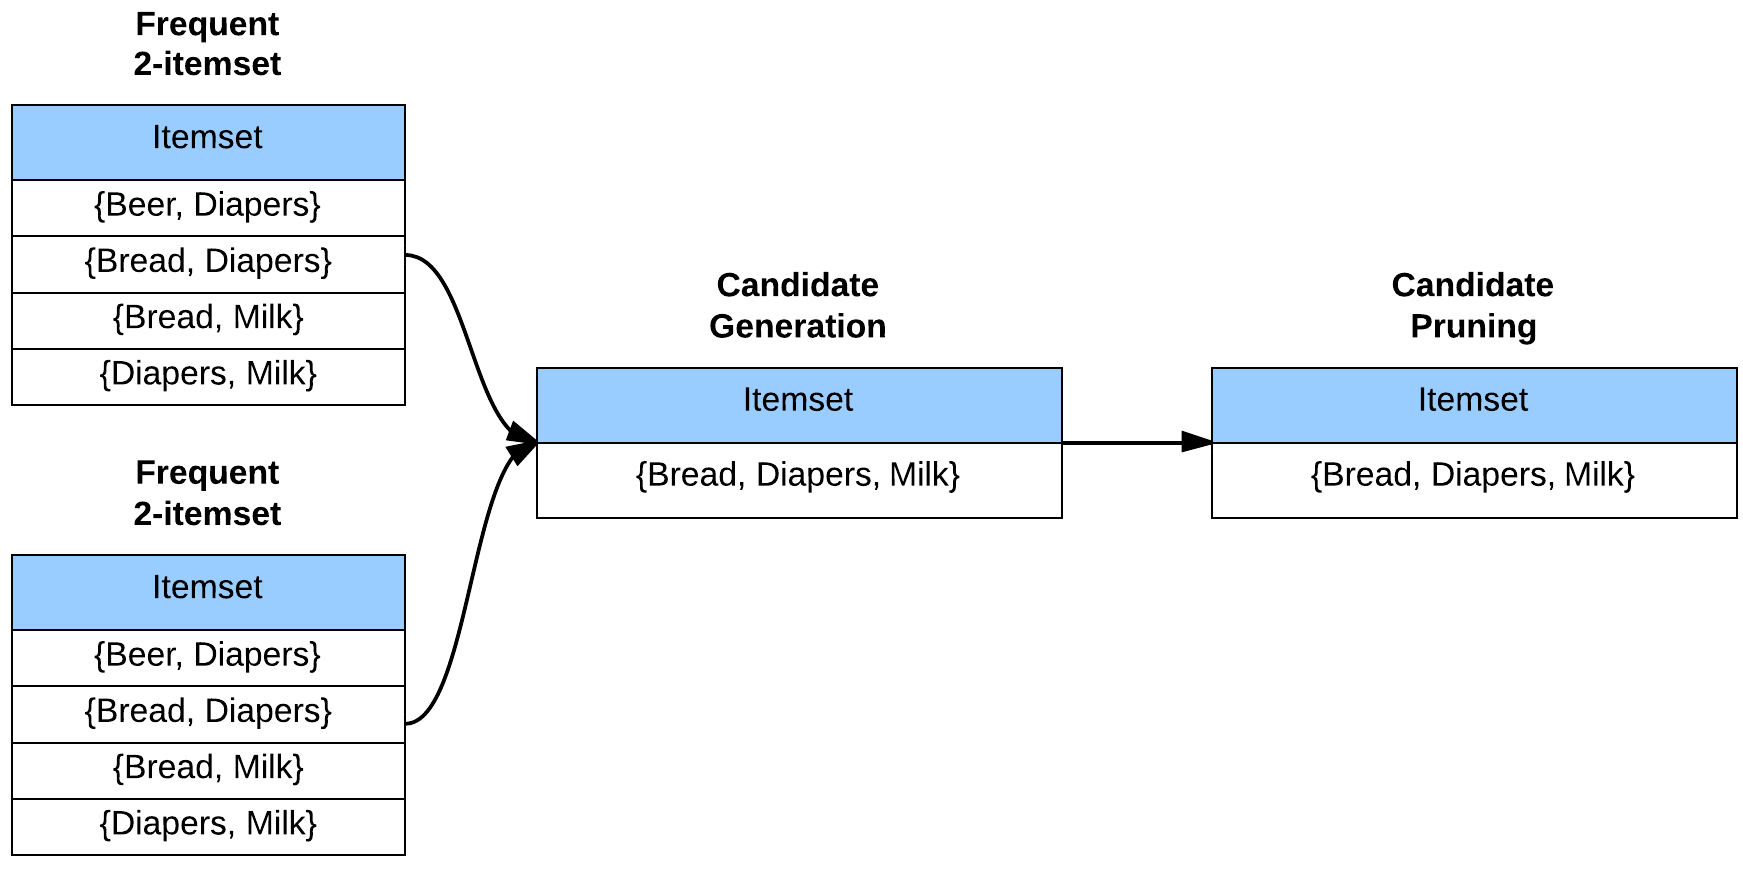
\includegraphics[width=\textwidth]{pics/apriori3.png}
					\caption{$F_{k-1} \times F_{k-1}$ illustration}
				\end{figure}

	\clearpage
	\section{Support Counting}

	Support counting is the process of determining the frequency of occurance for every candidate itemset
	that survives the candidate pruning step of the apriori-gen function. 

	One approach for doing this is to compare each transaction against very candidate itemset and 
	to update the support counts of candidates contained in the transaction. 

	An alternative approach is to enumerate the itemsets contained in each 
	transaction and use them  to update the support counts of their respective candidatee itemsets.
	
		\begin{figure}[H]
		\centering
		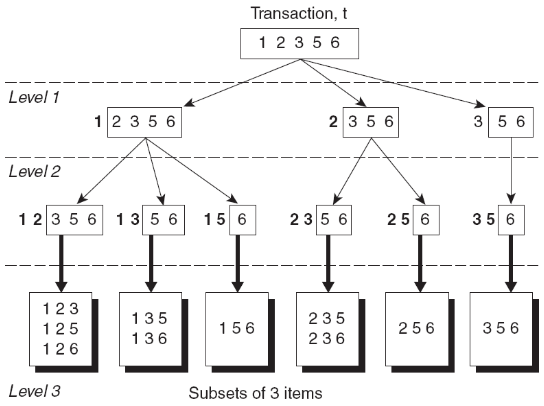
\includegraphics[scale=0.5]{pics/enumerateSubsets.png}
		\caption{Enumerating subsets of three items from a transaction t}
		\end{figure}

	In the Apriori algorithm, candidate itemsets are partitioned into different buckets and stored
	in a hash tree. During support counting, itemsets contained in each transaction are also hashed 
	into their appropriate buckets. That way, instead of comparing each itemset in the transaction 
	with every candidate itemset, it is matched only against candidate itemsets that belong to the 
	same bucket. 

		\begin{figure}[H]
			\centering
			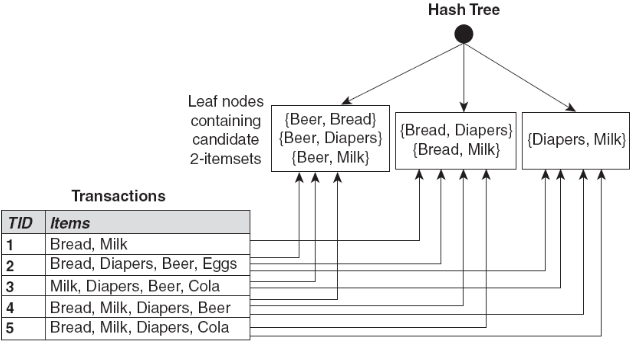
\includegraphics[scale=0.5]{pics/supportCount.png}
			\caption{Counting support of itemsets using hash structure}
		\end{figure}

		\begin{figure}[H]
			\centering
			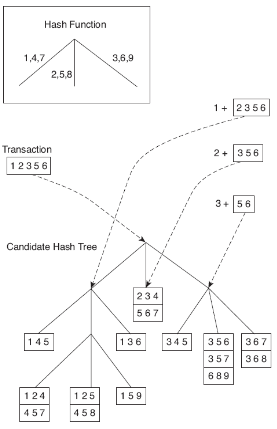
\includegraphics[scale=0.6]{pics/hash.png}
			\caption{Hasing a transaction at the root node of a hash tree}
		\end{figure}

	\section{Computational Complexity}

	The computational complexity of the apriori algorithm can be affected by the following factors:

		\begin{itemize}
			\item {\bf Support Threshold:} lowering the support threshold often results in more
			itemsets being declared as frequent. More frequent itemsets gives more comparisions in
			the algorithm.
			\item {\bf Number of items (Dimensionality):} As the number of items increases, more
			space will be needed to store the support counts of items. 
			\item {\bf Number of transactions:} since the apriori algorithm makes repeated passes
			over the data set, its run time increases with a large number of transactions. 
			\item {\bf Average transaction width:} this affects the Apriori algorithm in two ways.
			First, the maximum  size of frequent itemsets tends to increase as the 
			average transaction width increases. As a result, more candiadate itemsets must be
			examined during candidate generation and support counting.
			Second, as the transaction width increases. more
			itemsets are contained in the transaction. This will increase the number of hash 
			tree traversals performed during support counting.
			\item {\bf Generation of frequent 1-itemsets:} for each transaction, we need to 
			update the support count for every item present in the transaction.
			\item {\bf Candidate generation} 
			\item {\bf Support counting} 
		\end{itemize}




	\clearpage
	\section{Rule Generation}

		This section describes how to extract association rules efficiently from a given 
		frequent itemset. 

		{\bf Theorem:} {\it If a rule X $\rightarrow$ Y - X does not satisfy the confidence
		threshold, then any X' $\rightarrow$ Y - X', where X' is a subset of X, must not satisfy
		the confidence threshold as well.}

		\subsection*{Rule generation in Apriori Algorithm}

		The Apriori algorithm uses a level-wise approach for generating association rules, 
		where each level corresponds to the number of items that belong to the rule 
		consequent. Initially, all the high-confidence rules that have only one item
		in the rule consequent are extracted. These rules are then used to generate
		new candidate rules.

		{\bf Example:} if \{acd\} $\rightarrow$ \{b\} and \{abd\}$\rightarrow$\{c\} are
		high-confidence rules, then the candidate rule \{ad\} $\rightarrow$ \{bc\} is
		generated by merging the consequents of both rules. 
		
		Suppose the confidence for \{bcd\} $\rightarrow$ \{a\} is low. All the rules
		containing item a in its consequent, including \{cd\} $\rightarrow$ \{ab\},
		\{bd\} $\rightarrow$ \{ac\}, \{bc\} $\rightarrow$ \{ad\}, and \{d\} $\rightarrow$ \{abc\}
		can be discarded.

		\begin{figure}[H]
			\centering
			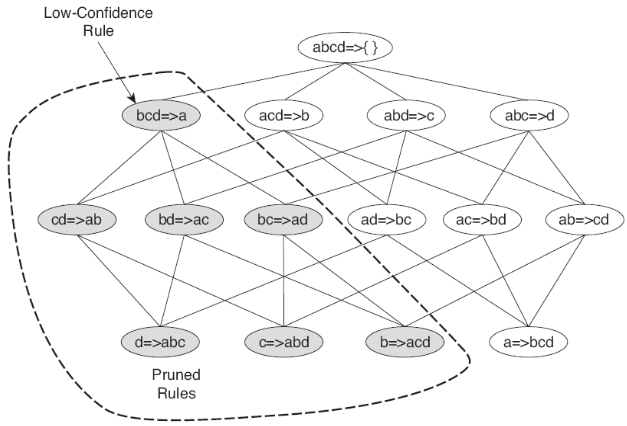
\includegraphics[width=\textwidth]{pics/prune.png}
			\caption{Pruning of association rules using the confidence measure}
		\end{figure}

	\clearpage
	\section{Compact Representation of Frequent Itemsets}
		In practice, the number of frequent itemsets produced from a transaction data set
		can be very large. It is useful to identify a samll representative set of itemsets
		from which all other frequent itemsets can be derived. 
		Two such representations are presented in this section in the form of maximal and
		closed frequent itemsets.

		\subsection{Maximal Frequent Itemsets}

		{\bf Maximal Frequent Itemsets:} a maximal frequent itemset is defined as a frequent
 		itemset for which none of its immidiate supersets are frequent.

 			\begin{figure}[H]
 				\centering
 				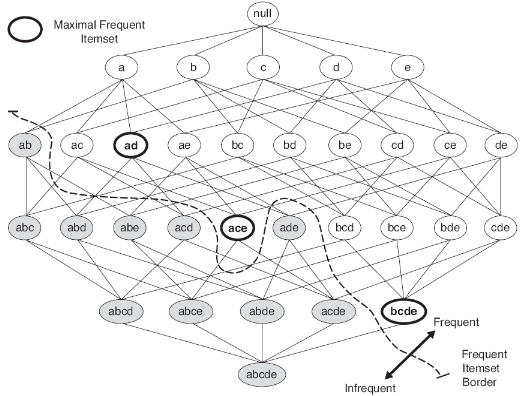
\includegraphics[scale=0.6]{pics/maximal.png}
 			\end{figure}

 		Maximal frequent itemsets form the smallest set of itemsets from which all frequent 
 		itemsets can be derived. For example, the frequent itemsets shown in figure ...
 		can be divided into two groups:

 		\begin{itemize}
 			\item Frequent itemsets that begin with item a and that may contain items
 			c, d, or e. This group includes itemsets such as \{a\}, \{a,c\}, \{a,d\},
 			\{a,e\}, and \{a,c,e\}.
 			\item Frequent itemsets that begin with items b, c, d or e. This group
 			includes itemsets such as \{b\}, \{b,c\}, \{c,d\}, \{b,c,d,e\}, etc.
 		\end{itemize}

 		\clearpage
 		\subsection{Closed Frequent Itemsets} 

 			Closed itemsets provide a minimal representation of itemsets without losing
 			their support information.

 			{\bf Closed Itemset:} {\it An itemset X is closed if none of its immidiate supersets has
 			exactly the same support count as X. }

 			{\bf Closed Frequent Itemsets:} {\it An itemset is a closed frequent itemset
 			if it is closed and its support is greater than or eaqual to minsup.}
 			\begin{figure}[H]
 				\centering
 				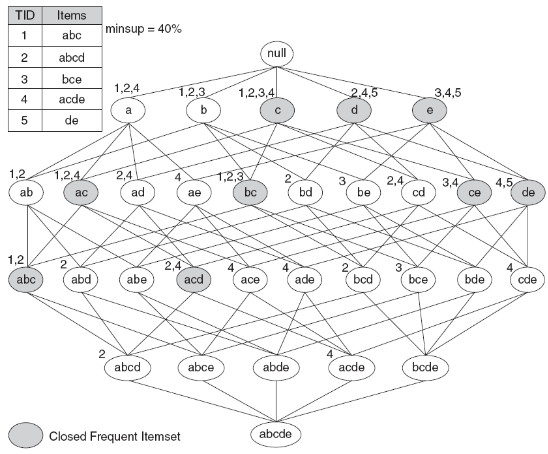
\includegraphics[scale=0.6]{pics/closed.png}
 				\caption{An example of the closed frequent itemsets (minsup = 40\%)}
 			\end{figure}

 			In figure 6.13 we have associated each node (itemset) in the lattice with a list
 			of its corresponding transaction IDs. For example, since the node \{b,c\} is
 			associated with transaction IDs 1,2 and 3, its support count is equal to 3. 

 			\begin{figure}[H]
 				\centering
 				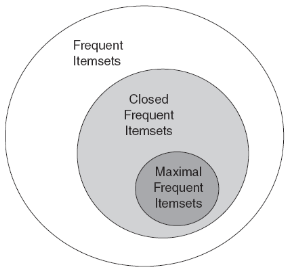
\includegraphics[scale=0.5]{pics/relationship.png}
 				\caption{Relationships among frequent, maximal frequent, and closed maximal frequent itemsets}
 			\end{figure}


 	\section{Alternative Methods for Generating Frequent Itemsets}

 		Several alternative methods have been developed to overcome these limitations of the,
 		and improve upon the efficiency of the Apriori algorithm. The following is a high-level
 		description of these methods:

 		\subsection{Traversal of Itemset Lattice}

 		Different search strategies in  traversal on a itemset lattice:
 		
 		{\bf General-to-specific vs. Specific-to-general:} The apriori 
 			algorithm uses a general-to-specific search strategy, where pairs of
 			frequent (k-1)-itemsets are merged to obtain candidate k-itemsets.
 			The difference between these is wether you start the search on the top
 			or on the bottom. You can use a {\bf bidirectional} where you start in both
 			ends and meets in the middle. 

 			\begin{figure}[H]
 				\centering
 				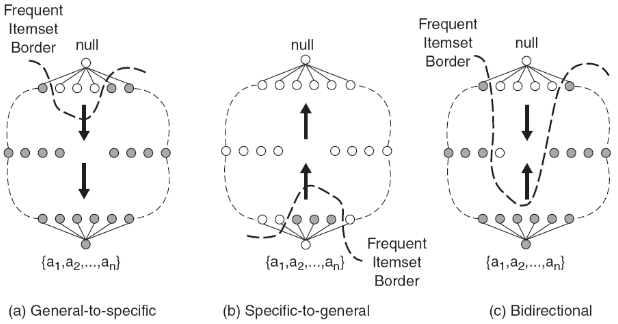
\includegraphics[scale=0.5]{pics/traversal.png}
 				\caption{General-to-specific, Specific-to-general, and bidirectional search}
 			\end{figure}
 		
 		{\bf Equivalence Clases:} Another way to envision the traversal is to
 			first partition the lattice into disjoint groups of nodes (or equivalence classes).
 			A frequent itemset generation algorithm searches for frequent itemsets within
 			a particualar equivalence class before moving to another equivalence class. 
 			Equivalence classes can be defined according to the {\bf prefix} of {\bf suffix} labels of 
 			an itemset. In this case, two itemsets belong to the same equivalence class if 
 			they share a common prefix or suffix of length k.

 			\begin{figure}[H]
 				\centering
 				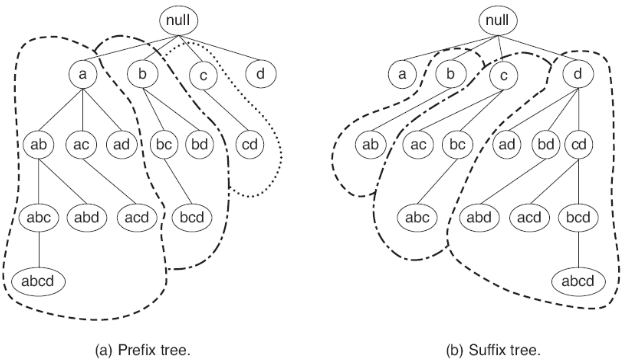
\includegraphics[scale=0.36]{pics/equvivalence.png}
 				\caption{Equvivalence classes based on the prefix and suffix labels of itemsets}
 			\end{figure}

 		{\bf Breadth-First vs. Depth-First:} The Apriori algorithm traverses the lattice in a breadth-first
 		manner. It first discovers all the frequent 1-itemsets, followed by the frequent 2-itemsets,
 		and so on, until no new frequent itemsets are generated. The itemset lattice ccan also be
 		traversed in a depth-first manner.

 		\begin{figure}[H]
 				\centering
 				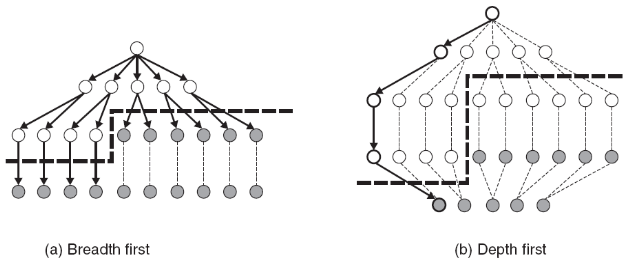
\includegraphics[scale=0.5]{pics/bfdf.png}
 				\caption{Breadth-first and depth-first straversals}
 		\end{figure}

 		\subsection{Representation of Transaction Data Set}

 			There are many ways to represent a transaction data set. The choice of representation can 
 			affect the I/O costs incurred when computing the support of candidate itemsets.
 			One way is a {\bf horizontal data layout}, and is used in the Apriori algorithm.
 			Another possibility is to store the list of transaction identifiers associated with
 			each item. Such representation is known as the {\bf vertical data layout}.

 		\begin{figure}[H]
 				\centering
 				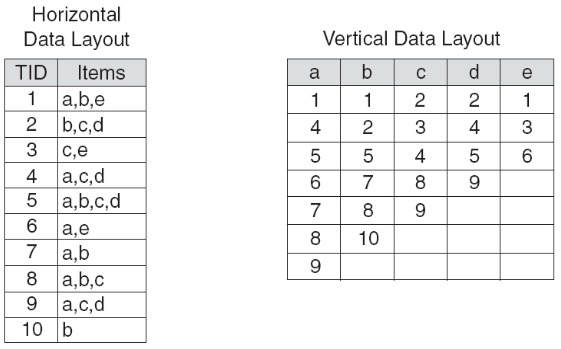
\includegraphics[scale=0.5]{pics/horizontal.png}
 				\caption{Horizontal and vertical data format}
 		\end{figure}

 	\clearpage
 	\section{FP-Growth Algorithm}

 		This section represents an alternative algorithm called {\bf FP-growth} that takes
 		a radically different approach to discovering frequent itemsets. This algorithm
 		encodes the data set using a compact data structure called an {\bf FP-tree} and
 		extracts frequent itemsets directly from this structure. 

 		{\bf FP-tree representation:} An FP-tree is a composed representation of the input data.
 		It is constructed by reading the data set one transaction at a time and mapping each
 		transaction onto the path in the FP-tree. As different transactions can have several items 
 		in common, their paths may overlap. 
 		Each node in the tree contains the label of an item along with a counter that shows
 		the number of transactions mapped onto the given path. 

 		\begin{enumerate}
 			\item The data set is scanned once to determine the support count of each item.
 			Infrequent items are discarded, while the frequent items  are sorted in decreasing
 			support count. For the data set in the figure, a is the most frequent item, 
 			followed by b, c, d and e.
 			\item The algorithm makes a second pass over the data to construct the tree.
 			After reading the first transaction, \{a,b\}, the nodes labeled as a and b are created.
 			A path is then formed from null $\rightarrow$ a $\rightarrow$ b to endcode
 			the transaction. Every node along the path has now a frequency count of 1.
 			\item The process of adding each transaction to a path and increasing the count along
 			the path continues until every transaction has been mapped onto one of the paths in the 
 			FP-tree. The final result is given in figure 6.19. 
 		\end{enumerate}
 		
 		\begin{figure}[H]
 				\centering
 				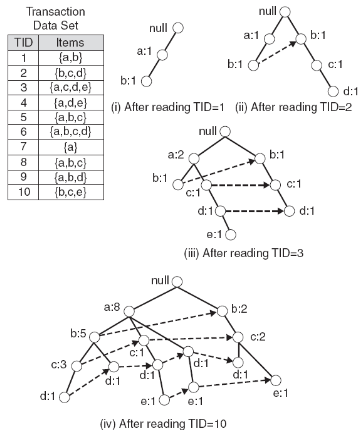
\includegraphics[scale=0.7]{pics/fptree.png}
 				\caption{Constructing of an FP-tree}
 		\end{figure}


 	\section{Evaluation of Association Patterns}


 		{\bf \Huge \color{red} PENSUM ???}